\subsection{Endoplasmic Reticulum}
    Endoplasmic reticulum (ER) is a network of membranes inside a cell through which proteins and other molecules move. Ribosomes are small and round organelles with the main function to produce the protein needed for the cell. They are located in a continuos membrane system that forms a series of flattened sacs, this membrane is called ER (see Figure \ref{fig:cell}) (\cite{er}). ER itself is moslty located around the nuclei. In order to stain ER were treated with Donkey Anti-Rabbit IgG antibody. This is a fluorescent stain that binds strongly with ER. Its analysis is also important for the CLD as this organelle directly related to the process of protein production within the cell: ER is responsible for the synthesis, folding, modification, and transport of proteins (\cite{er_2}). The proximity of the ER to the nucleus allows essentially controls the protein production. For example, when the protein os misfolded or incorrectly folded it will accumulate in the ER lumen and will serve as a signal to activate misfolded protein response. In contrast to other imaging datasets ER dataset does not require special preprocessing step as the images were of a good quality without any visible problems (see the ground truth image in Figure \ref{fig:er-combined}).
    
    \subsubsection{Training and predictions}
        During the training with PCC loss the model has successfully converged already after 35 epochs, however a clear overfit was encountered (see Figure \ref{fig:er-overfit} (left)) with the best PCC loss before the overfit being $0.0713$. Overfitting happens due to the lack of data, as for ER case there were much fewer samples than for nuclei for example (see Table \ref{table:data}). Even though one could use early-stopping approach and simply choose an earlier epoch before overfit, the better approach would be to use regularization methods described in section \ref{section:regularization}. Additional regularization in terms of data augmentations was introduced. The new learning curve is shown in Figure \ref{fig:er-overfit} (middle). Overfit happens now much later (after $120$ epochs) and PCC loss improves to $0.0701$. Introducing a stronger regularization with the use of weight decay in adadelta optimizer and dropout layers with a dropout rate of $0.1$ (see Figure \ref{fig:er-overfit} (right)) reduces the overfit completely, however at the same time increases the loss to $0.099$.
\begin{figure}[H]
	\begin{center}
		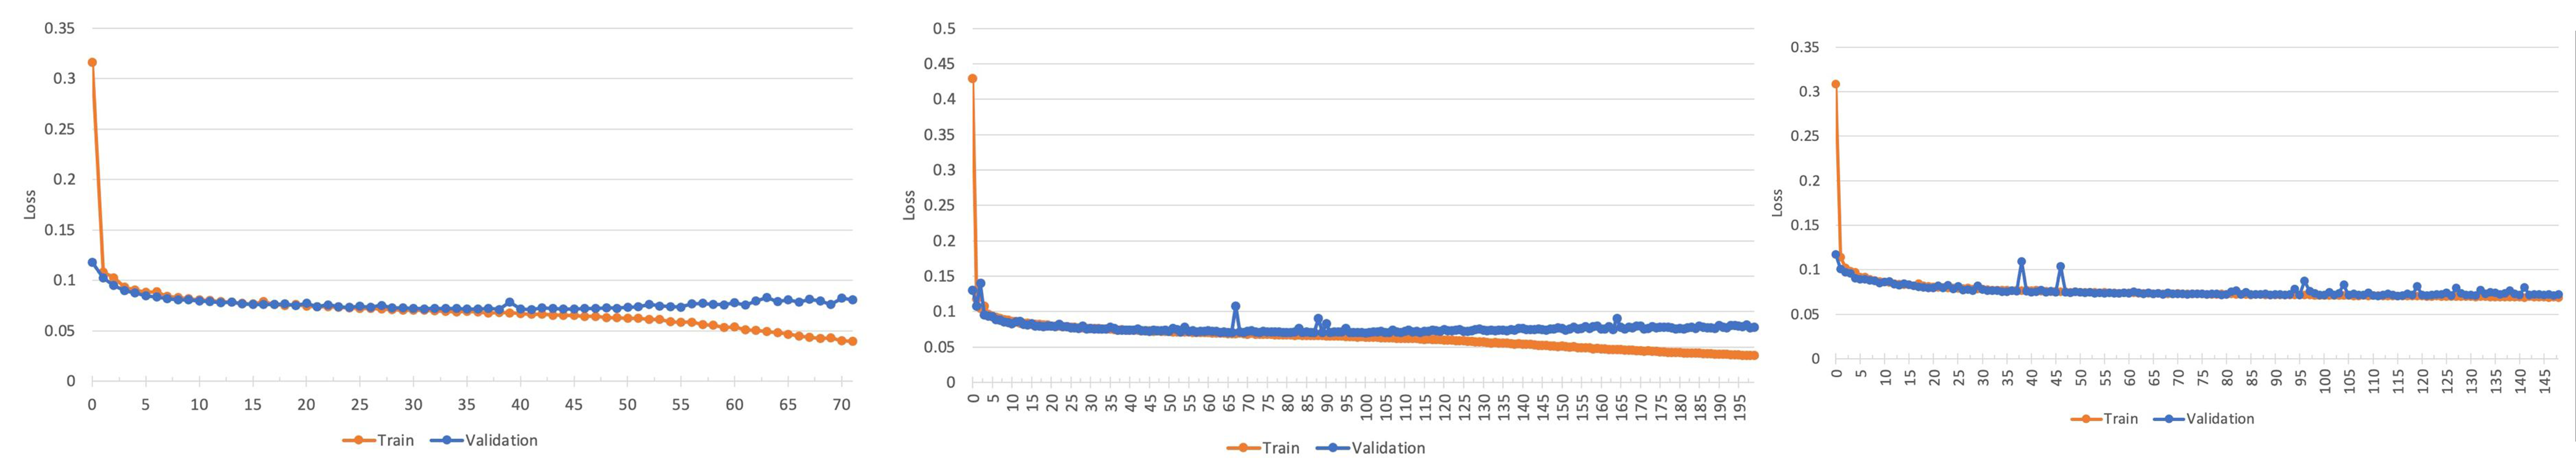
\includegraphics[width=\linewidth]{bilder/ER/segmentation/reg-not-reg.png}
		\caption{Default model (left), slightly regularized model(middle), strongly regularized model (right)}\label{fig:er-overfit}
	\end{center}
\end{figure}

Although the validation loss seem to be higher in comparison to $0.0701$, in this case the growths were not explained by the difference between the validation sets, where the loss was measured on. PCC losses on the same validation set for both were $0.0701$ and $0.0742$. It might have been the case that the regularization was too strong. In this case it would be better to use early-stopping approach with the epoch that has the lowest loss.
    \subsubsection{Combination of nuclei and actin predictions}
        Now having two models for the predictions of two organelles: nuclei and ER, it is interesting to visualize the predictions together (see Figure \ref{fig:er-combined}). It is clear from the image that ER indeed is located around the nucleus. As one can see, there is a great advantage in the used of \textit{in silico} fluroescence labeling especially for the cases where several cell targets have to be ananlysed. Instead of a expesive and time-consuming procedure for staining several targets at the same time they can be predicted based on one DIC image only.
\begin{figure}[htb]
    \centering
    \setkeys{Gin}{width=\linewidth}
    \centering
        \begin{tabularx}{\textwidth}{YYYY}
            (a)  \textbf{Ground truth} &
            (b)  \textbf{Prediction} &
            (c)  \textbf{Prediction + nuclei} \\
            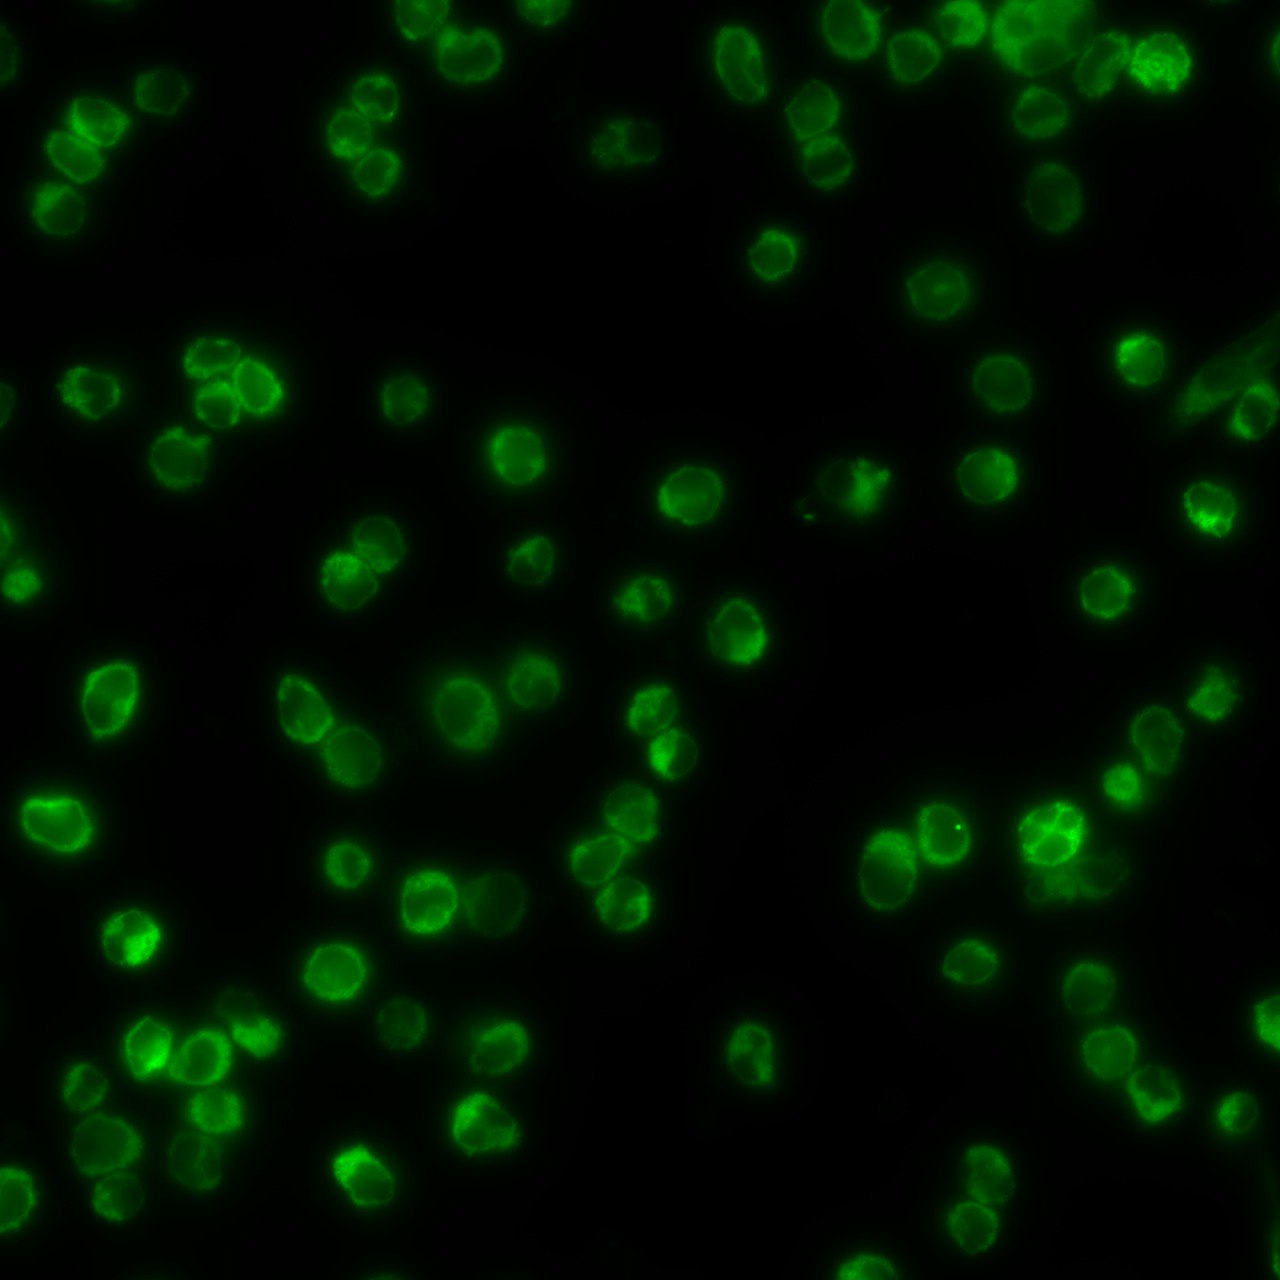
\includegraphics{bilder/ER/gt.jpg} & 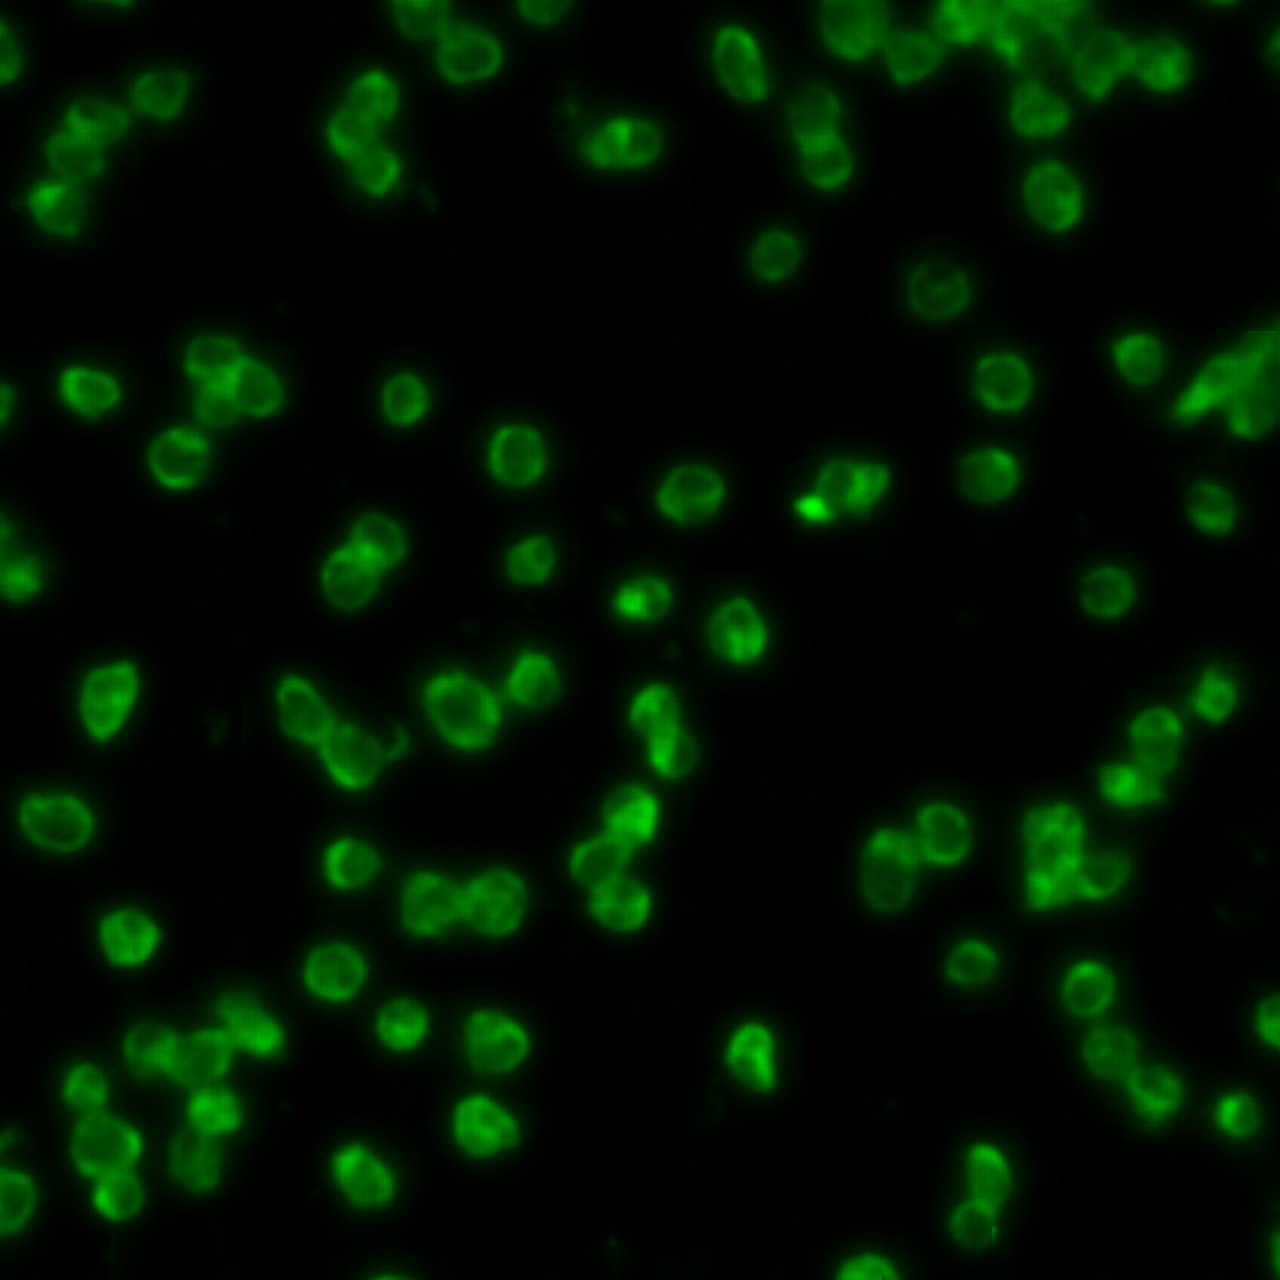
\includegraphics{bilder/ER/er.jpg} &
            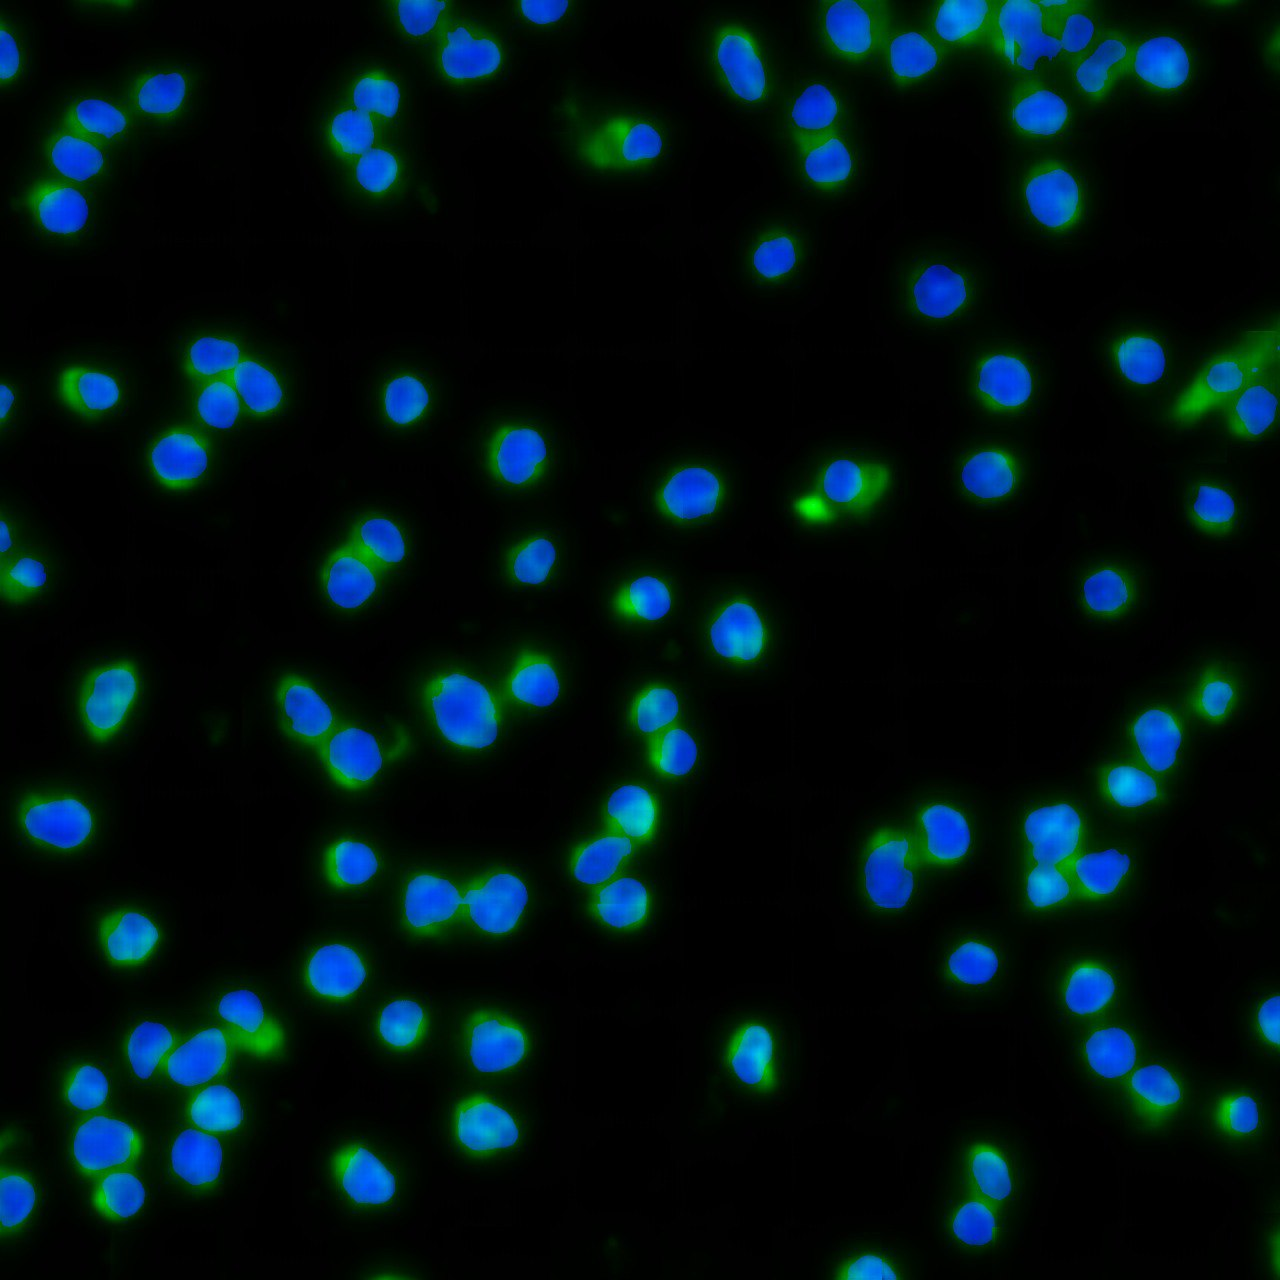
\includegraphics{bilder/ER/gt_nuclei.jpg}
        \end{tabularx}
    \caption{Combination of ER with nuclei prediction. Image (a) here is the original fluorescence image of ER, image (b) is the UNet prediction of ER and image (c) is the combination of predicted ER (green) with predicted nuclei (blue).}
    \label{fig:er-combined}
\end{figure}
    \subsubsection{Postprocessing for ER segmentation}
        The process of ER fluorescence segmentation is somewhat different in comparison to nuclei segmentation. These fluorescence staining has a stronger "shining" around the ER itself and therefore any method for background removal would be helpful to reduce it. One of such methods based on the rolling ball algorithm is described in more details in section \ref{par:background-removal}.

Initially it was established that a local thresholding approach for segmentation would be nessecary here as well, as the images also have a non-uniform illumitation. However a downside of a local thresholding algorithm is the appearance of the artifacts briefly mentioned in the previous section and presented in Figure \ref{fig:artifacts-er}. Even though the background in fluorescence imaging appears to be completely black, it still contains some slight signal (non-zero values), that are boosted by a local threshold and becomes an unwanted artifact. 
\begin{figure}[H]
	\begin{center}
		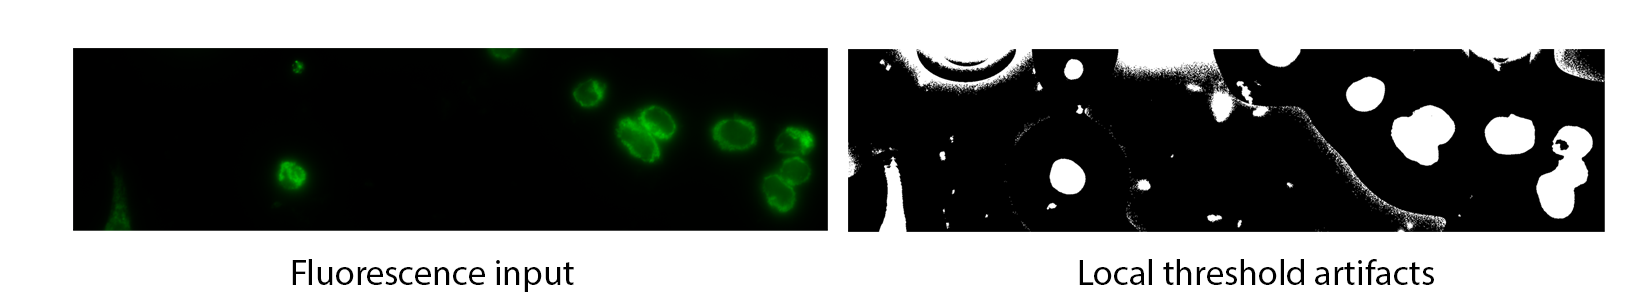
\includegraphics[width=\linewidth]{bilder/ER/artifacts.png}
		\caption{Artifacts from local thresholding algorithm}\label{fig:artifacts-er}
	\end{center}
\end{figure}
Such falsely recognized regions appeared in the nuclei as well, yet there they were easily filtered out based on the shape criteria. All nuclei are almost round and convex objects, whereas background artifacts are prolonged completely non-convex objects. Unfortunately, such filtration cannot be applied to ER imaging as very often ER from one cell is located very close one to the ER from another cell, and together they may form a long non-convex object, that now could not be filtered out this easily. That is why it is very important to remove the background noise here first before applying a local threshold.

In order to do that one can first apply a rough "over-predictive" global thresholding, that will cover a true signal fully, including the "shine" around the ER, but will ignore the background noise. In the role of "over-predictove" global mean thresholding algorithm can be used (see Figure \ref{fig:er-segmentation-steps}.2). The mask created with the mean thresholding approach is used to zero out all the pixels that are not covered by it. And after that the local thresholding can be successfully applied with the \textit{block\_size} of $181$ (Figure \ref{fig:er-segmentation-steps}.4). Then  algorithm fills in all the holes in the middle of ER that might have appeared during the thresholding. Morphological opening (see Section TODO cite section) and Gaussian Blur with the squared kernel $3 \times 3$ are applied. Connected components are detected afterwards and filtered based on the limit of the area they occupy, this filters out mostly very small components from the mask which might be produced by the left out background noise. The whole algorithm overview is described below:

Segmentation steps are described in Algorithm \ref{alg:er-segmentation-steps} and also illustrated in Figure \ref{fig:er-segmentation-steps}.

\begin{algorithm}
    \caption{Fluorescence segmentation}
    \begin{algorithmic}
    \item 1. Normalize image
    \item 2. Apply global \textit{threshold\_mean} to receive initial mask.
    \item 3. Zero out pixels outside the mask
    \item 4. Apply local thresholding.  
    \item 5. Apply \textit{fill\_holes} transformation.
    \item 6. Morphological opening from OpenCV and Gaussian blur.
    \item 7. Run \textit{findContours} from OpenCV in order to obtain separate regions and filter out too small regions.
    \end{algorithmic}
    \label{alg:er-segmentation-steps}
\end{algorithm}    

\begin{figure}[htb]
    \begin{center}
        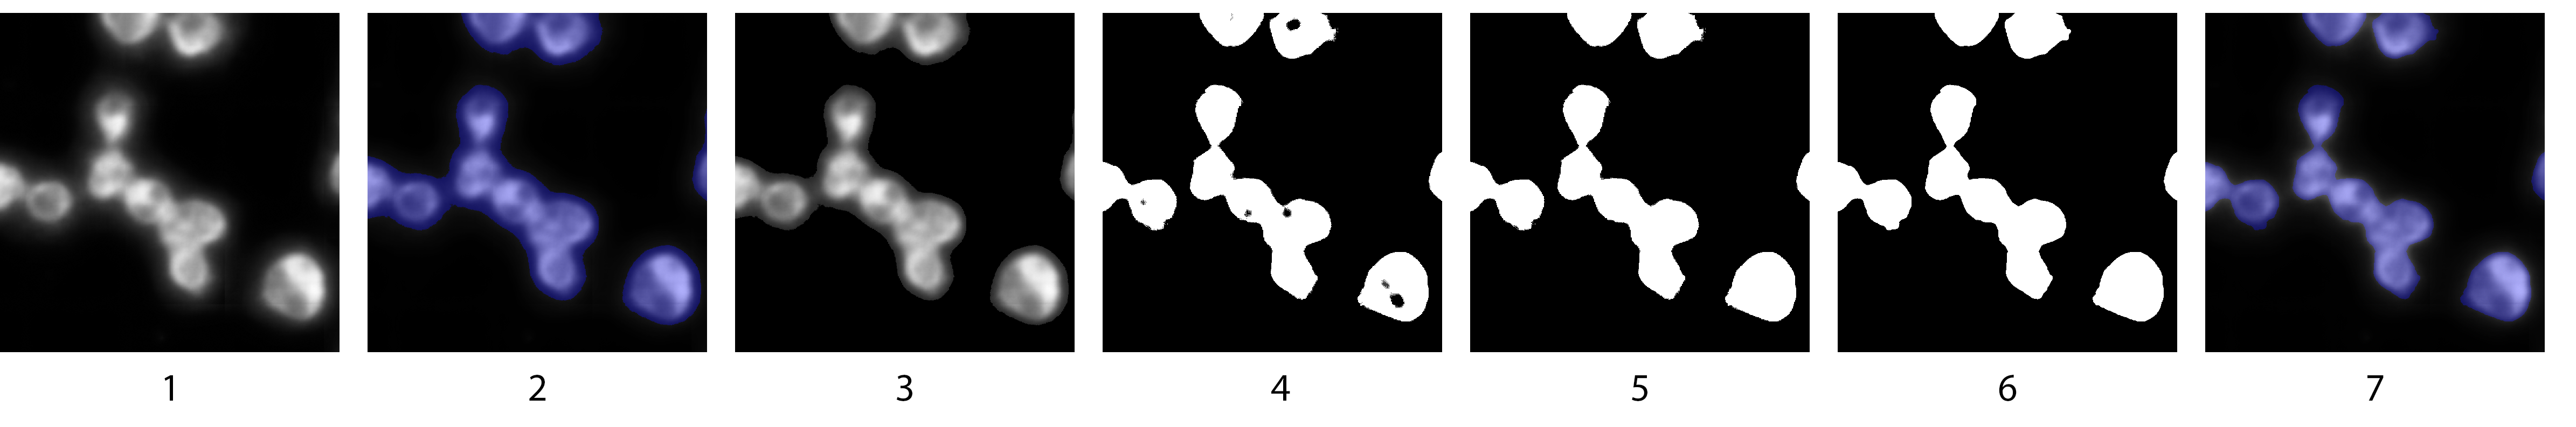
\includegraphics[width=\linewidth]{bilder/ER/segmentation/segmentation.png}
        \caption{Segmentation steps in ER postprocessing}\label{fig:er-segmentation-steps}
    \end{center}
\end{figure}
    \subsubsection{Conclusions}
        Training the model on the ER stain images produced very successful results that can be used as a replacement for manual staining with \textit{in silico} labeling. Overfit of the model has been encountered and several experiments were performed to overcome it, the best checkpoint was selected and evaluated.

The segmentation of ER for further downstream metrics evaluation was proposed. The problem of overlap between cells being present was discovered, which causes the segmented regions to merge together. Subsequently, a better preprocessing algorithm was proposed. This algorithm helps to avoid the artifacts appearing from a local thresholding.

The combination of ER with nuclei predictions was visualized and analysed, it was confirmed that the models produce realistic results confirming biological definition of their mutual arrangement within the cell. However, it is recommended to test the models using the simultaneous staining of both organelles to get quantitative metrics of the accuracy.
    \subsubsection{Generalizability across phenotypes}
        TODO move into the other section, there is only 1 phenotype here
        TODO train the model on one phenotype and predict on the other, compare predictions (visually?) 
        postprocessing with metrics then?
        Add metrics

    